% !TEX program = xelatex
\documentclass[UTF8,fontset=fandol,a4paper,11pt]{ctexart}
\usepackage[margin=21mm,top=23mm,bottom=22mm,headheight=16pt]{geometry}
\usepackage{amsmath,amssymb,mathtools,bm}
\usepackage{tikz}
\usetikzlibrary{arrows.meta,calc,angles,quotes,patterns}
\usepackage{xcolor,booktabs,array,longtable,enumitem,fancyhdr,needspace}
\usepackage[unicode,hidelinks]{hyperref}
\definecolor{ink}{HTML}{24343C}
\definecolor{accent}{HTML}{166A70}
\definecolor{muted}{HTML}{65747A}
\definecolor{rulegray}{HTML}{D4DDE0}
\definecolor{warm}{HTML}{966037}
\color{ink}
\setlength{\parindent}{2em}
\setlength{\parskip}{4pt}
\linespread{1.12}
\AtBeginDocument{\setlength{\abovedisplayskip}{6pt plus 2pt minus 1pt}
\setlength{\belowdisplayskip}{6pt plus 2pt minus 1pt}
\setlength{\abovedisplayshortskip}{0pt plus 1pt}
\setlength{\belowdisplayshortskip}{4pt plus 1pt}}
\setlist[enumerate]{label=(\arabic*),leftmargin=2.3em,itemsep=3pt,topsep=4pt}
\setlist[itemize]{leftmargin=2em,itemsep=2pt,topsep=4pt}
\allowdisplaybreaks[1]
\setlength{\emergencystretch}{2em}
\setcounter{secnumdepth}{0}
\providecommand{\tightlist}{\setlength{\itemsep}{0pt}\setlength{\parskip}{0pt}}
\ctexset{section={format=\Large\bfseries\color{accent},beforeskip=10pt,afterskip=9pt},
subsection={format=\normalsize\bfseries\color{accent},beforeskip=10pt,afterskip=4pt},
subsubsection={format=\normalsize\bfseries,beforeskip=8pt,afterskip=3pt}}
\pagestyle{fancy}
\fancyhf{}
\fancyhead[L]{\small\color{muted}物理学难题集萃}
% 页眉仅保留书名；版本名称只在封面显示。
\fancyfoot[L]{\small\color{muted}\chapterlabel}
\fancyfoot[R]{\small\thepage}
\renewcommand{\headrulewidth}{0.4pt}
\renewcommand{\footrulewidth}{0pt}
\newcommand{\dd}{\mathop{}\!\mathrm{d}}
\newcommand{\vect}[1]{\bm{#1}}
\newcommand{\tagline}[1]{\noindent{\small\color{muted}#1}\par}
\newcommand{\result}[1]{\begin{equation*}\boxed{#1}\end{equation*}}
\newcommand{\figcaption}[1]{\par\vspace{2pt}{\small\color{muted}#1}\par}
\newcommand{\teach}[2]{\Needspace{4\baselineskip}\subsection*{讲解要点与追问}#1\par\smallskip\noindent\textbf{追问：}#2\par}
\newcommand{\workarea}{\par\vspace{7mm}\noindent{\small\color{muted}作答区}\par\vspace{4mm}
\noindent\textcolor{rulegray}{\rule{\linewidth}{0.3pt}}\par\vspace{16mm}
\noindent\textcolor{rulegray}{\rule{\linewidth}{0.3pt}}\par\vspace{16mm}
\noindent\textcolor{rulegray}{\rule{\linewidth}{0.3pt}}\par\vspace{16mm}
\noindent\textcolor{rulegray}{\rule{\linewidth}{0.3pt}}}
\tikzset{axis/.style={-{Stealth[length=2mm]},thin,color=muted},
motion/.style={-{Stealth[length=2.3mm]},thick,color=accent},
force/.style={-{Stealth[length=2.3mm]},thick,color=warm},
traj/.style={thick,color=accent},guide/.style={dashed,thin,color=muted},
object/.style={thick,color=ink},every node/.style={font=\small}}\widowpenalty=10000\clubpenalty=10000\displaywidowpenalty=10000\newcommand{\chapterlabel}{光学试题}







\hypersetup{pdftitle={光学试题·学生版},pdfauthor={}}

\begin{document}\pdfbookmark[0]{光学试题}{cover}

\thispagestyle{empty}\vspace*{22mm}

\noindent{\Huge\bfseries 物理学难题集萃}\par\vspace{12mm}

\noindent{\LARGE 光学试题}\par\vspace{12mm}

\noindent{\Large\color{accent}学生版}\par\vspace{9mm}

\noindent\textcolor{accent}{\rule{\linewidth}{1pt}}\par\vspace{9mm}

\noindent 第1--6题\par\vfill\clearpage

\pdfbookmark[1]{题目目录}{contents}\section*{题目目录}

\begin{longtable}{@{}r p{113mm} r@{}}\toprule 题号 & 题目 & 页码\\\midrule

\hyperref[q:1]{1} & \hyperref[q:1]{有限共轭点的无像差凹面反射镜} & \pageref{q:1} \\

\hyperref[q:2]{2} & \hyperref[q:2]{双透镜成像与中间像处的场镜} & \pageref{q:2} \\

\hyperref[q:3]{3} & \hyperref[q:3]{惠更斯与冉斯登目镜的主点和焦点} & \pageref{q:3} \\

\hyperref[q:4]{4} & \hyperref[q:4]{切接透镜的干涉条纹与有限重叠区} & \pageref{q:4} \\

\hyperref[q:5]{5} & \hyperref[q:5]{双层膜三束反射光的相消与最薄组合} & \pageref{q:5} \\

\hyperref[q:6]{6} & \hyperref[q:6]{棱镜色散与衍射限制的分辨本领} & \pageref{q:6} \\

\bottomrule\end{longtable}

\clearpage

\pdfbookmark[2]{第 1 题 有限共轭点的无像差凹面反射镜}{q1}

\section*{第 1 题\quad 有限共轭点的无像差凹面反射镜}\label{q:1}


凹面反射镜顶点为$O$，轴上物点$Q$与$O$距离为$s>0$，要求从$Q$出发、落在反射面上的光线经一次反射后均会聚于轴上$Q'$；$Q'$与$O$距离为$s'>0$，两点在顶点同侧。反射面连通、光滑并包含顶点附近的一片区域，周围介质均匀。

以$O$为坐标原点、由物点一侧指向顶点的方向为$+x$，取$Q=(-s,0)$、$Q'=(-s',0)$。根据费马原理求子午截线方程、中心、长短半轴，并写出旋转曲面的方程；说明所得面为何满足反射定律。


\begin{center}\begin{minipage}{.98\linewidth}\centering
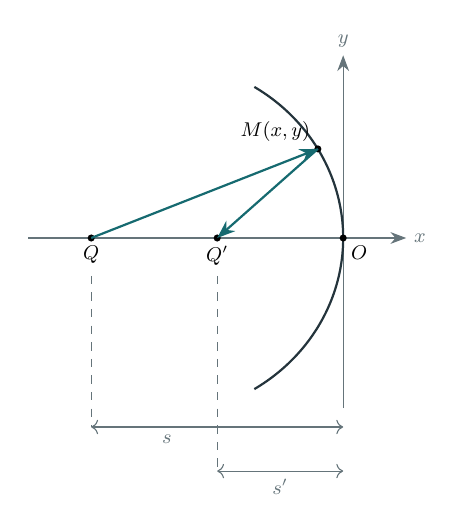
\begin{tikzpicture}[scale=.8,transform shape]

\draw[axis] (-5,0)--(1,0) node[right] {$x$};
\draw[axis] (0,-2.7)--(0,2.9) node[above] {$y$};
\draw[object,domain=-58:58,samples=100] plot ({-3+3*cos(\x)},{2.828427*sin(\x)});
\coordinate (Q) at (-4,0);\coordinate (V) at (-2,0);\coordinate (M) at (-.401924,1.414214);
\fill (Q) circle (1.6pt) node[below] {$Q$};
\fill (V) circle (1.6pt) node[below] {$Q'$};
\fill (0,0) circle (1.6pt) node[below right] {$O$};
\fill (M) circle (1.6pt) node[above left] {$M(x,y)$};
\draw[motion] (Q)--(M);\draw[motion] (M)--(V);
\draw[guide] (-4,-.6)--(-4,-3);\draw[guide] (-2,-.6)--(-2,-3.7);
\draw[axis,<->] (-4,-3)--(0,-3) node[pos=.3,below] {$s$};
\draw[axis,<->] (-2,-3.7)--(0,-3.7) node[midway,below] {$s'$};

\end{tikzpicture}
\figcaption{图光试.1\quad 两有限共轭点在顶点同侧，落到凹面上的光线反射后会聚。}
\end{minipage}\end{center}

\par\vspace{5mm}\noindent{\small\color{muted}作答区}\par\vspace{3mm}\noindent\textcolor{rulegray}{\rule{\linewidth}{0.3pt}}\par\vspace{12mm}\noindent\textcolor{rulegray}{\rule{\linewidth}{0.3pt}}

\clearpage

\pdfbookmark[2]{第 2 题 双透镜成像与中间像处的场镜}{q2}

\section*{第 2 题\quad 双透镜成像与中间像处的场镜}\label{q:2}


沿光轴依次放置两块会聚薄透镜$L_1,L_2$，焦距均为$10\,\mathrm{cm}$，间距$70\,\mathrm{cm}$。物在$L_1$前$20\,\mathrm{cm}$处。
\begin{enumerate}
\item 求最后像的位置、横向放大率及正倒。
\item 在两镜之间增加有限正焦距薄透镜$L_3$，使最后像的位置仍保持不变，确定其位置。
\item 结合特殊光线说明$L_3$怎样使一部分被$L_2$孔径挡住的离轴光重新参与成像；说明增加透镜的集光作用所需的孔径条件。
\end{enumerate}
采用傍轴近似，忽略透镜吸收；分别讨论最后像的位置和孔径传光量。


\begin{center}\begin{minipage}{.98\linewidth}\centering
\begin{tikzpicture}[scale=.8,transform shape]

\draw[axis] (-2.8,0)--(9,0) node[right] {$x$};
\draw[object,<->] (0,-1.8)--(0,1.8) node[above] {$L_1,\ f_1=10\,\mathrm{cm}$};
\draw[object,<->] (7,-1.8)--(7,1.8) node[above] {$L_2,\ f_2=10\,\mathrm{cm}$};
\draw[motion] (-2,0)--(-2,.6) node[above] {物};
\draw[axis,<->] (-2,-1)--(0,-1) node[midway,below] {$20\,\mathrm{cm}$};
\draw[axis,<->] (0,-2.2)--(7,-2.2) node[midway,below] {$70\,\mathrm{cm}$};

\end{tikzpicture}
\figcaption{图光试.2\quad 两会聚透镜的已知焦距、间距与物距。}
\end{minipage}\end{center}

\par\vspace{5mm}\noindent{\small\color{muted}作答区}\par\vspace{3mm}\noindent\textcolor{rulegray}{\rule{\linewidth}{0.3pt}}\par\vspace{12mm}\noindent\textcolor{rulegray}{\rule{\linewidth}{0.3pt}}

\clearpage

\pdfbookmark[2]{第 3 题 惠更斯与冉斯登目镜的主点和焦点}{q3}

\section*{第 3 题\quad 惠更斯与冉斯登目镜的主点和焦点}\label{q:3}


目镜由场镜$L_1$和接目镜$L_2$组成，两者均为会聚薄透镜，焦距分别为$f_1,f_2$，间距$d$，前后均为空气。光从左向右，取$L_1$位置为$x=0$、$L_2$为$x=d$。
\begin{enumerate}
\item 惠更斯目镜满足$f_1:f_2:d=3:1:2$；令$f_2=a$，求有效焦距、物方主点$H$、像方主点$H'$、物方焦点$F$及像方焦点$F'$的绝对坐标。
\item 冉斯登目镜满足$f_1:f_2:d=1:1:2/3$；令$f_1=f_2=a$，求相同各量。
\item 哪一种可将物体放在整组透镜之前，当作普通放大镜使用？结合物方焦点位置说明。
\end{enumerate}
采用傍轴近似，所有位置统一用向右为正的$x$坐标表达。


\begin{center}\begin{minipage}{.98\linewidth}\centering
\begin{tikzpicture}[scale=.85,transform shape]

\draw[axis] (-1,0)--(8,0) node[right] {$x$};
\draw[object,<->] (0,-1.5)--(0,1.5) node[above] {$L_1$};
\draw[object,<->] (6,-1.5)--(6,1.5) node[above] {$L_2$};
\node[below] at (0,-1.5) {$x=0$};\node[below] at (6,-1.5) {$x=d$};
\draw[axis,<->] (0,-2.5)--(6,-2.5) node[midway,below] {$d$};
\node at (3,2.6) {光从左向右；两侧介质均为空气};

\end{tikzpicture}
\figcaption{图光试.3\quad 先固定坐标，再计算组合系统的主点和焦点。}
\end{minipage}\end{center}

\par\vspace{5mm}\noindent{\small\color{muted}作答区}\par\vspace{3mm}\noindent\textcolor{rulegray}{\rule{\linewidth}{0.3pt}}\par\vspace{12mm}\noindent\textcolor{rulegray}{\rule{\linewidth}{0.3pt}}

\clearpage

\pdfbookmark[2]{第 4 题 切接透镜的干涉条纹与有限重叠区}{q4}

\section*{第 4 题\quad 切接透镜的干涉条纹与有限重叠区}\label{q:4}


一焦距$f=20\,\mathrm{cm}$的薄凸透镜，从中央切去宽为$a$的条带，再把剩下两半向中间平移并粘接。两半的光心相距$a$，粘接后的总直径为$D=2.0\,\mathrm{cm}$。波长$\lambda=500\,\mathrm{nm}$的单色点光源$S$位于粘接体的中心轴线上，距透镜为$f$。透镜另一侧放置垂直中心轴的屏，测得条纹间距$\Delta y=0.20\,\mathrm{mm}$。
\begin{enumerate}
\item 求切去条带的宽度$a$。
\item 屏距透镜多远时，可见重叠区内的条纹数最多？给出中央纵截面内重叠宽度随屏距的变化。
\end{enumerate}
采用傍轴几何光学描述光束外缘，在两束的重叠区域计算干涉；忽略边缘衍射对外缘的模糊。


\begin{center}\begin{minipage}{.98\linewidth}\centering
\begin{tikzpicture}[scale=.7,transform shape]

\draw[object] (-1,1.9)..controls(-1.8,.5)and(-1.8,-.5)..(-1,-1.9);
\draw[object] (-1,1.9)..controls(-.2,.5)and(-.2,-.5)..(-1,-1.9);
\fill[white] (-1.9,-.4) rectangle (-.1,.4);
\draw[guide] (-1.65,.4)--(-.35,.4);\draw[guide] (-1.65,-.4)--(-.35,-.4);
\draw[axis,<->] (-2.2,-.4)--(-2.2,.4) node[midway,left] {$a$};
\draw[motion] (0,0)--(1,0);
\draw[object] (2,1.5)..controls(1.3,.3)and(1.3,-.3)..(2,-1.5);
\draw[object] (2,1.5)..controls(2.7,.3)and(2.7,-.3)..(2,-1.5);
\draw[object] (1.5,0)--(2.5,0);
\draw[axis,<->] (3,-1.5)--(3,1.5) node[midway,right,yshift=4pt] {$D$};
\begin{scope}[xshift=6cm]
\draw[axis] (-2.5,0)--(3.5,0);
\fill (-2,0) circle (1.8pt) node[above] {$S$};
\draw[object,<->] (0,-1.5)--(0,1.5);
\draw[object] (3,-2)--(3,2) node[above] {屏};
\draw[axis,<->] (-2,-2.3)--(0,-2.3) node[midway,below] {$f$};
\draw[axis,<->] (0,-2.9)--(3,-2.9) node[midway,below] {$z$};
\end{scope}

\end{tikzpicture}
\figcaption{图光试.4\quad 中央去条带后平移粘接，D指粘接后的总口径。}
\end{minipage}\end{center}

\par\vspace{5mm}\noindent{\small\color{muted}作答区}\par\vspace{3mm}\noindent\textcolor{rulegray}{\rule{\linewidth}{0.3pt}}\par\vspace{12mm}\noindent\textcolor{rulegray}{\rule{\linewidth}{0.3pt}}

\clearpage

\pdfbookmark[2]{第 5 题 双层膜三束反射光的相消与最薄组合}{q5}

\section*{第 5 题\quad 双层膜三束反射光的相消与最薄组合}\label{q:5}


玻璃基底上依次涂两层透明薄膜，空气、第一层、第二层、基底折射率分别为$n_0,n_1,n_2,n_3$，满足$n_0<n_1<n_2$且$n_2>n_3$。膜厚分别为$t_1,t_2>0$。真空波长$\lambda$的单色光垂直入射。

在只保留三个界面各反射一次所形成的三束反射光、忽略更高次内部反射的模型中，三束到达共同参考面的振幅大小相等。欲使它们叠加后的反射强度为零，先使$t_1$最小，再在这个$t_1$下使$t_2$最小，求该厚度组合；给出相位分支，比较两种最小化顺序对应的厚度组合。


\begin{center}\begin{minipage}{.98\linewidth}\centering
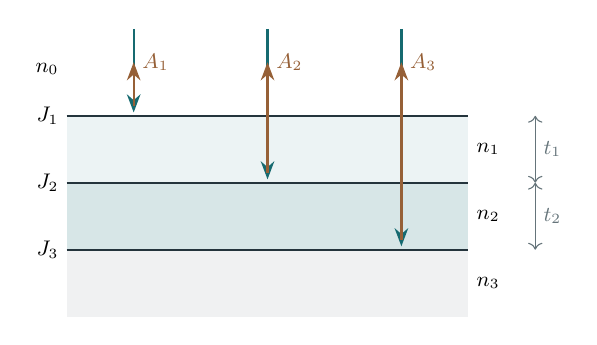
\begin{tikzpicture}[scale=.85,transform shape]

\fill[accent!8] (-3,1) rectangle (3,2);
\fill[accent!17] (-3,0) rectangle (3,1);
\fill[muted!10] (-3,-1) rectangle (3,0);
\foreach \y/\p in {2/J_1,1/J_2,0/J_3}{\draw[object] (-3,\y)--(3,\y);\node[left] at (-3,\y) {$\p$};}
\node[left] at (-3,2.7) {$n_0$};
\node[right] at (3,1.5) {$n_1$};\node[right] at (3,.5) {$n_2$};
\node[right] at (3,-.5) {$n_3$};
\draw[axis,<->] (4,1)--(4,2) node[midway,right] {$t_1$};
\draw[axis,<->] (4,0)--(4,1) node[midway,right] {$t_2$};
\draw[motion] (-2,3.3)--(-2,2.05);
\draw[motion] (0,3.3)--(0,1.05);
\draw[motion] (2,3.3)--(2,.05);
\draw[force] (-2,2.15)--(-2,2.8) node[right] {$A_1$};
\draw[force] (0,1.15)--(0,2.8) node[right] {$A_2$};
\draw[force] (2,.15)--(2,2.8) node[right] {$A_3$};

\end{tikzpicture}
\figcaption{图光试.5\quad 三条法向反射路径分列表示，$n_0<n_1<n_2,\ n_2>n_3$。}
\end{minipage}\end{center}

\par\vspace{5mm}\noindent{\small\color{muted}作答区}\par\vspace{3mm}\noindent\textcolor{rulegray}{\rule{\linewidth}{0.3pt}}\par\vspace{12mm}\noindent\textcolor{rulegray}{\rule{\linewidth}{0.3pt}}

\clearpage

\pdfbookmark[2]{第 6 题 棱镜色散与衍射限制的分辨本领}{q6}

\section*{第 6 题\quad 棱镜色散与衍射限制的分辨本领}\label{q:6}


棱镜光谱仪中的等腰三棱镜$ABC$顶角为$\beta$，底边$BC=L$，两腰长为$b$，材料折射率为$n(\lambda)$。中心波长$\lambda$的光在最小偏向角条件下通过棱镜，入射面$AB$被均匀、充分照明。

把有限入射面视为宽度$b$的单缝，考虑它对出射主峰的衍射展宽，按瑞利判据推导分辨本领$\mathcal R=\lambda/\delta\lambda$。保留入射、折射角和有效投影孔径的关系，说明色散率符号如何处理。

采用窄谱带一阶近似和夫琅禾费衍射模型，忽略狭缝宽度、像差及探测器像素造成的其他展宽。


\begin{center}\begin{minipage}{.98\linewidth}\centering
\begin{tikzpicture}[scale=.8,transform shape]

\coordinate (A) at (0,3);\coordinate (B) at (-2,0);\coordinate (C) at (2,0);
\fill[accent!8] (A)--(B)--(C)--cycle;\draw[object] (A)--(B)--(C)--cycle;
\node[above] at (A) {$A$};\node[below left] at (B) {$B$};\node[below right] at (C) {$C$};
\node at (0,2.25) {$\beta$};
\node[left] at (-1.3,1.7) {$b$};\node[right] at (1.3,1.7) {$b$};
\draw[axis,<->] (-2,-.8)--(2,-.8) node[midway,below] {$L$};

\draw[motion] (-4,.565)--(-1,1.5)--(1,1.5)--(4,.565);
\node at (0,4) {等腰棱镜，中心波长按最小偏向通过};

\end{tikzpicture}
\figcaption{图光试.6\quad 满照面宽与底边长度不同，中心光路关于顶角平分线对称。}
\end{minipage}\end{center}

\par\vspace{5mm}\noindent{\small\color{muted}作答区}\par\vspace{3mm}\noindent\textcolor{rulegray}{\rule{\linewidth}{0.3pt}}\par\vspace{12mm}\noindent\textcolor{rulegray}{\rule{\linewidth}{0.3pt}}

\end{document}
